%
% DS 7180 Readings Template
%
\documentclass[12pt]{article}

%
% Packages
%
\usepackage{amsmath}
\usepackage{amssymb}
\usepackage{amsthm}
\usepackage{enumerate}
\usepackage{graphicx}


%
% Package settings
%

%
% Document Settings
%
\setlength{\parskip}{1pc}
\setlength{\parindent}{0pt}
\setlength{\topmargin}{-3pc}
\setlength{\textheight}{9.5in}
\setlength{\oddsidemargin}{0pc}
\setlength{\evensidemargin}{0pc}
\setlength{\textwidth}{6.5in}


%
% Document Macros
%
\newcommand{\reals}{\rm I\!R}

\graphicspath{{imgs/}}

% START DOCUMENT
\begin{document}

\section{Problem Statement}

How can we use zero-shot and transfer learning to
better denoise images? 

\section{Deep Learning Book}

Relevant chapters from DLB \cite{Goodfellow-et-al-2016}

\begin{itemize}
\item \textbf{7.7 Multitask Learning}
  \begin{itemize}
  \item The model can generally be divided into two kinds
    of parts and associated parameters:
    \begin{enumerate}
    \item Task-specific parameters (which only benefit the examples
      of their task to achieve good generalization). These are the
      upper layers of the neural network in figure 7.2
    \item Generic parameters, shared across all the tasks (which benefit
      from the pooled data of all the tasks). These are the lower
      layers of the neural network in figure 7.2
    \end{enumerate}
  \item From the point of view of deep learning, the underlying prior
    belief is the following: \textit{among the factors that explain the
      variations observed in the data associated with the different
      tasks, some are shared across two or more tasks.}
  \end{itemize}
\item \textbf{7.13 Adversarial Training}
  \begin{itemize}
  \item Adversarial examples also provide a means of accomplishing
    semi-supervised learning
  \item Approach encourages the classifier to learn a function that
    is robust to small changes anywhere along the manifold where
    the unlabeled data lie
  \item The assumption motivating this approach is that different
    classes usually lie on the disconnected manifolds, and a small
    perturbation should not be able to jump from one class manifold
    to another class manifold
  \end{itemize}
\item \textbf{15 Representation Learning}
  \begin{itemize}
  \item Training with supervised learning techniques on the labeled
    subset often results in severe overfitting
  \item Semi-supervised learning offers the chance to resolve this
    overfitting problem by also learning from the unlabeled data
  \item Specifically, we can learn good representations for the
    unlabeled data, and then use these representations to solve the
    supervised learning task
  \end{itemize}
\item \textbf{15.2 Transfer Learning and Domain Adaptation}
  \begin{itemize}
  \item The learner must perform two or more different tasks,
    but we assume that many of the factors that explain the variations
    in $P_1$ are relevant to the variations that need to be captured
    for learning $P_2$
  \item Typically understood in a supervised learning context, where the
    input is the same but the target may be of a different nature
  \item Two extreme forms of transfer learning are \textit{one-shot learning}
    and \textit{zerof-shot learning}, sometimes also called
    \textit{zero-data learning}.
    \begin{itemize}
    \item Only one labeled example of the transfer task is given for
      one-shot learning, while no labeled examples are given at all for
      the zero-shot learning task
    \item Zero-data learning \cite{larochelle2008} and zero-shot learning
      \cite{Palatucci:2009:ZLS:2984093.2984252, socher2013zeroshot}
      \end{itemize}
    \end{itemize}
\end{itemize}

\section{Papers}

\subsection{Zero-Shot Learning}

\begin{itemize}
\item CleanNet: Transfer Learning for Scalable Image Classifier Training
  With Label Noise \cite{Lee_2018_CVPR}
  \begin{itemize}
  \item In this paper, we study the problem of learning image
    classification models with label noise. Existing approaches
    depending on human supervision are generally not scalable as
    manually identifying correct or incorrect labels is time-consuming,
    whereas approaches not relying on human supervision are scalable but
    less effective. To reduce the amount of human supervision for label
    noise cleaning, we introduce CleanNet, a joint neural embedding network,
    which only requires a fraction of the classes being manually verified to
    provide the knowledge of label noise that can be transferred to other
    classes. We further integrate CleanNet and conventional convolutional
    neural network classifier into one framework for image classification
    learning. We demonstrate the effectiveness of the proposed algorithm on
    both of the label noise detection task and the image classification
    on noisy data task on several large-scale datasets. Experimental
    results show that CleanNet can reduce label noise detection error
    rate on held-out classes where no human supervision available by
    41.5\% compared to current weakly supervised methods. It also
    achieves 47\% of the performance gain of verifying all images with
    only 3.2\% images verified on an image classification task. Source
    code and dataset will be available at kuanghuei.github.io/CleanNetProject.
  \end{itemize}
\end{itemize}

\subsection{Image Denoising}

\begin{itemize}
\item \textbf{Deep Learning for Image Denoising: A Survey} \cite{tian2018deep}
  \begin{itemize}
  \item Since the proposal of big data analysis and Graphic Processing
    Unit (GPU), the deep learning technology has received a great deal
    of attention and has been widely applied in the field of imaging
    processing. In this paper, we have an aim to completely review and
    summarize the deep learning technologies for image denoising proposed
    in recent years. Morever, we systematically analyze the conventional
    machine learning methods for image denoising. Finally, we point out
    some research directions for the deep learning technologies in image
    denoising.
  \item \textit{4.1 The challenges of deep learning technologies in
    image denoising}
    \begin{enumerate}
    \item Current deep learning denoising methods only deal with AWGN,
      which are not effective for real noisy images, such as low light
      images.
    \item They can't use a model to deal with all the low level vision
      taks, such as image denoising, image super-resolution, image
      blurring, and image deblocking.
    \item They can't use a model to address the blind Gaussian noise
    \end{enumerate}
  \end{itemize}

\item \textbf{Correction by Projection: Denoising Images with Generative
  Adversarial Networks} \cite{DBLP:journals/corr/abs-1803-04477}
  \begin{itemize}
  \item Generative adversarial networks (GANS) transform low-dimensional
    latent vectors into visually plausible images. If the real dataset
    contains only clean images, then ostensibly, the manifold learned by the
    GAN should contain only clean images. In this paper, we propose to
    denoise corrupted images by finding the nearest point on the GAN
    manifold, recovering latent vectors by minimizing distances in image
    space. We first demonstrate that given a corrupted version of an image
    that truly lies on the GAN manifold, we can approximately recover the
    latent vector and denoise the image, obtaining significantly higher
    quality, comparing with BM3D. Next, we demonstrate that latent vectors
    recovered from noisy images exhibit a consistent bias. By subtracting
    this bias before projecting back to image space, we improve denoising
    results even further. Finally, even for unseen images, our method performs
    better at denoising than BM3D. Notably, the basic version of our method
    (without bias correction) requires no prior knowledge on the noise
    variance. To achieve the highest possible denoising quality, the best
    performing signal processing based methods, such as BM3D, require an
    estimate of the blur kernel.
  \end{itemize}
\item \textbf{Very Deep Convolutional Networks for Large-Scale Image
  Recognition} \cite{DBLP:journals/corr/SimonyanZ14a}
  \begin{itemize}
  \item In this work we investigate the effect of the convolutional network
    depth on its accuracy in the large-scale image recognition setting. Our
    main contribution is a thorough evaluation of networks of increasing
    depth using an architecture with very small (3x3) convolution filters,
    which shows that a significant improvement on the prior-art
    configurations can be achieved by pushing the depth to 16-19 weight
    layers. These findings were the basis of our ImageNet Challenge 2014
    submission, where our team secured the first and the second places in
    the localisation and classification tracks respectively. We also show
    that our representations generalise well to other datasets, where they
    achieve state-of-the-art results. We have made our two best-performing
    ConvNet models publicly available to facilitate further research on the
    use of deep visual representations in computer vision.
  \end{itemize}
\item \textbf{Universal Denoising Networks : A Novel CNN Architecture for
  Image Denoising} \cite{DBLP:journals/corr/abs-1711-07807}
  \begin{itemize}
  \item We design a novel network architecture for learning discriminative
    image models that are employed to efficiently tackle the problem of
    grayscale and color image denoising. Based on the proposed architecture,
    we introduce two different variants. The first network involves the
    convolutional layers as a core component, while the second one relies
    instead on non-local filtering layers and thus it is able to exploit the
    inherent non-local self-similarity property of natural images. As
    opposed to most of the existing deep network approaches, which require the
    training of a specific model for each considered noise level, the
    proposed models are able to handle a wide range of noise levels using a
    single set of learned parameters, while they are very robust when the
    noise degrading the latent image does not match the statistics of the noise
    used during training. The latter argument is supported by results that we
    report on publicly available images corrupted by uknown noise and which we
    compare against solutions obtained by competing methods. At the same
    time the introduced netowrks achieve excellent results under additive white
    Gaussian noise (AWGN), which are comparable to those of the current
    state-of-the-art network, while they depend on a more shallow architecture
    with the number of trained parameters being one order of magnitude
    smaller. These properties make the proposed netowrks ideal candidates to
    serve as sub-solvers on restoration methods that deal with general
    inverse imaging problems such as deblurring, demosaicking, superresolution,
    etc.
  \end{itemize}
\end{itemize}

\section{Suggestions from Rose}

Want to make sure we thoroughly understand the research papers
Rose suggested. It seems like she cares less about the application
and more about the process and technique. She's been advocating for
GANs and zero-shot learning (an extreme version of transfer learning).

Rose suggested ``Deep convolutional neural network for image deconvolution''
\cite{xu2014deep} which included their source code and dataset
(http://lxu.me/projects/dcnn/). She also recommended a more
recent paper, ``Image Inpainting via Generative Multi-column Convolutional Neural Networks'' \cite{wang2018image}.

\section{Relevant background from DLB}

First, I review DLB in CNN, then talk about where this paper
picks up.

\subsubsection*{9.1 The Convolution Operation}

Recall the Convolution Operation from DLB Section 9.1
\cite{Goodfellow-et-al-2016}.

\[
s(t) = \int x(a)w(t-a) da. \tag{9.1}
\]

where $x(t)$ is a single output at time $t$. Both $x$ and $t$
are real-valued. We assume that our ability to measure $x(t)$
is done in a noisy way. We would like to average or take the
maximum (average pooling vs. max pooling I believe) of several
measurements to reduce this noise; with more weight given to
recent measurements. We can do this with a weighting
function $w(a)$ where $a$ is the age of the measurement. In
general, convolution is defined for any functions for which the
above integral is defined and may be used for other purposes besides
taking weighted averages. \newline

In convolutional network terminology, the first argument(in this
example, the function $x$) to the convolution is often referred
to as the \textbf{input}, and the second argument (in this
example, the function $w$) as the \textbf{kernel}. The output is
sometimes referred to as the \textbf{feature map}. If we now
assume that $x$ and $w$ are defined only on integer $t$, we can
define the discrete convolution:
\[
s(t) = (x * w)(t) = \sum_{a=\infty}^{\infty} x(a)w(t-a) \tag{9.3}
\]

\subsubsection*{9.3 Pooling}

A typical layer of a CNN consists of three stages (see figure 9.7). In
the first stage, the layer performs several convolutions in parallel to
produce a set of linear activations. In the second stage, each linear
activation is run through a nonlinear activation function, such as the
rectified linear (ReLU) activation function. The second stage is sometimes
called the \textbf{detector stage}. In the third stage, we use a
\textbf{pooling function} to modify the output of the layer further.

\begin{center}
  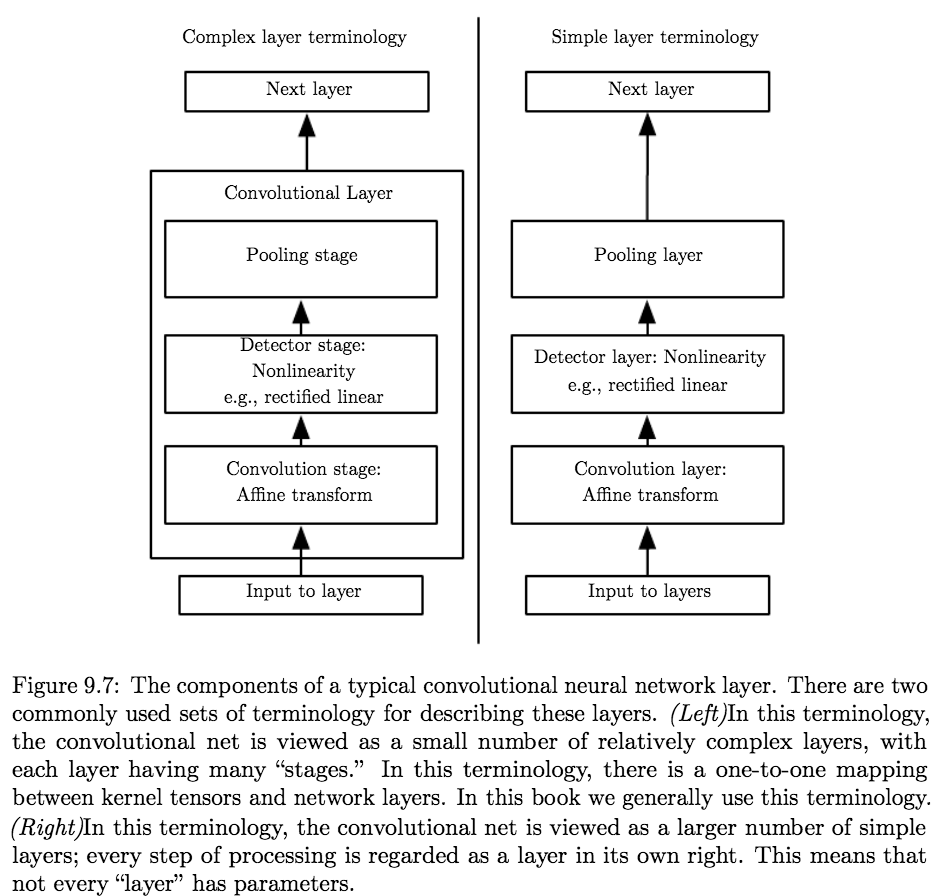
\includegraphics[scale=0.75]{fig9_7}
\end{center}

\subsubsection*{9.10 The Neuroscientific Basis for Convolutional Networks}

Focus on a part of the brain called V1, also known as the
\textbf{primary visual cortex}. A CNN is designed to capture
three properties of V1:

\begin{enumerate}
\item V1 is arranged in a spatial map. It actually has a two
  dimensional structure of the image in the retina.
\item V1 contains many \textbf{simple cells}. A simple cell's
  activity can to some extent be characterized by a
  \textit{linear function} of the image in a small, spatially
  localized receptive field. The detector units of a CNN are
  designed to emulate these properties of simple cells
\item V1 also contains \textbf{complex cells}. These cells respond
  to features that are similar to those detected by simple cells,
  but complex cells are invariant to small shifts in the position
  of the feature. This inspires the pooling units of CNNs.
\end{enumerate}

Simple cells are roughly linear and selective for certain features,
complex cells are more nonlinear and become invariant to some
transformations of these simple cell features, and stacks of
layers that alternate between selectivity and invariance can yield
'grandmother' cells for specific phenomena. A linear model can be
used to approximate a neuron's weights. This apporach is known as
\textbf{reverse correlation}. \newline

Reverse correlation shows us that most V1 cells have weights that
are defined by \textbf{Gabor functions}. The Gabor function describes
the weight at a 2-D point in the image. We can think of an image as
being a function of 2-D coordinates, $I(x,y)$. Likewise, we can
think of a simple cell as sampling the image at a set of locations,
defined by a set of $x$ coordinates $\mathbb{X}$ and a set of $y$
coordinates $\mathbb{Y}$, then applying weights that are also a
function of the location, $w(x,y)$. From this point of view, the
response of a simple cell to an image is given by
\[
s(I) = \sum_{x \in \mathbb{X}} \sum_{y \in \mathbb{Y}} w(x,y)I(x,y)
\tag{9.15}
\]

Specifically, $w(x,y)$ takes the form of a Gabor function:
\[
w(x,y;\alpha, \beta_x, \beta_y, f, \phi, x_0, y_0, \tau) =
\alpha \exp(-\beta_x x^{\prime 2} - \beta_y y^{\prime 2})
\cos(f x^{\prime} + \phi), \tag{9.16}
\]
where... see equations (9.17) and (9.18).... It has two important
factors: one is a Gaussian function, and the other ise a cosine
function. \newline

The Gaussian factor $\alpha \exp(-\beta_x x^{\prime 2} - \beta_y y^{\prime 2})$
can be seen as a gating term that ensures that the simple cell will
respond only to values near where $x^\prime$ and $y^\prime$ are both
zero, in other words, \text{near the center} of the cell's receptive
field. \newline

The cartoon view of a complex cell is that it computes the $L^2$ norm of
the 2-D vector containing two simple cells' responses:
$c(I) = \sqrt{s_0(I)^2 + s_1(I)^2}$.

\subsection{DCNN for Image Deconvolution \cite{xu2014deep} (2014)}

\begin{itemize}
\item We need to understand and recognize why CNNs use a linear
  model to approximate simple cells. Even when approximating a complex
  cell, it looks like they're just taking the difference of two linear
  simple cells. Xu et. al. \cite{xu2014deep} identify this property as
  a problem when denoising images
\item ``Real blur degradation seldom complies with an ideal linear
  convolution model due to camera noise, etc.\cite{xu2014deep}
\item Instead of perfectly modeling outliers, which is rather
  challenging from a \textit{generative} model perspective, we develop
  a deep CNN to capture characteristics of degradation
\item Our solution is to establish the connection between
  traditional optimization-based schemes and a neural network architecture
  where a novel, separable structure is introduced as a reliable support for
  robust deconvolution against artifacts.
\end{itemize}


\subsection{Gen CNN for Image Inpainting \cite{wang2018image} (2018)}

ok




\bibliographystyle{unsrt}
\bibliography{references}

\end{document}
